\documentclass[withoutpreface,bwprint]{cumcmthesis} %去掉封面与编号页
\usepackage[framemethod=TikZ]{mdframed}
\usepackage{url}   % 网页链接
\usepackage{subcaption} % 子标题、
\usepackage{graphicx}
\title{“信息引航者”——基于MGCA的信息推荐系统}
\usepackage{listings}
\lstset{language=Matlab}
\usepackage{pythonhighlight}
\usepackage{setspace}
\begin{document}
	
	\maketitle\thispagestyle{empty}
	\begin{abstract}
		信息技术不断发展,互联网上存在着大量信息,通过小红书、今日头条、bilibili等互联网平台获取信息是主要的信息获取途径之一。随着互联网上信息的越来越多,想要在海量信息中获取我们感兴趣或有需求的信息愈加困难。\par
		推荐系统的出现正是为了解决这种“信息过载”的问题。推荐系统已在互联网中得到了广泛的应用,并给应用它的企业带来了丰厚的利润。推荐系统给亚马逊带来了35\%的销售收入,给Netflix带来了高达75\%的消费,并且Youtube主页上60\%的浏览来自推荐服务。有关推荐系统的研究具有十分深远的意义与巨大的实用价值。\par
		
	\end{abstract}
	\setcounter{page}{1}
	\tableofcontents
	\newpage
	\section{引言}
	\subsection{研究背景及意义}
	\subsubsection{ 信息过载问题的解决迫在眉睫} 
	互联网高速发展,信息呈爆炸式增长,用户逐渐由信息匮乏时代迈入了信息过载时代——过量信息反而使得用户无法找到自己需要的信息。信息过载问题会产生一系列问题,比如用户体验变差、用户数量骤减、用户粘性降低等。
	信息爆炸的今天,个性化新闻推荐技术已经变成了许多新闻网站和App的关键技术。新闻的数据来源众多,可能一分钟就有成千上万条新的数据产生,在数据量激增的情况下,需要付出更多的人力成本,并且人工处理速度慢,效率十分低下。一套个性化新闻推荐系统刚好可以应用于有效缓解这种信息过载问题。如图1是新闻推荐系统通过个性化推荐实现精准化投放信息的流程示意。
	\begin{figure}[H]
		\centering
		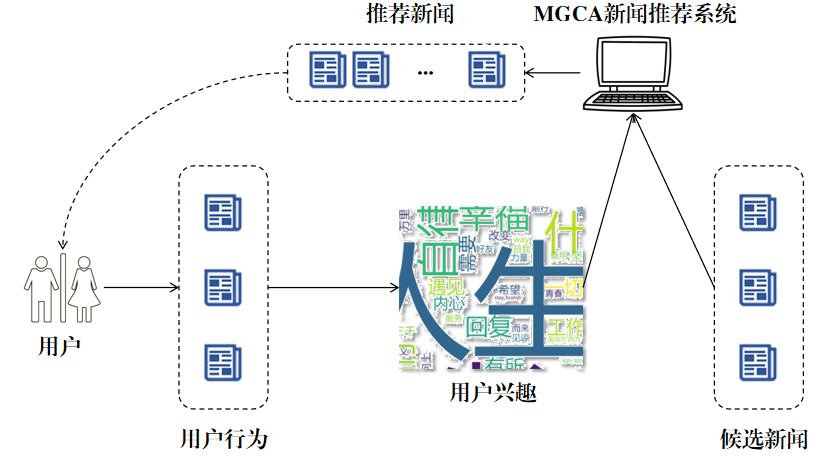
\includegraphics[width=0.95\textwidth]{2}
		\caption{个性化新闻推荐系统实现精准化投放信息}
		\label{fig:circuit-diagcam}
	\end{figure}
	\subsubsection{ 互联网与推荐系统的融合带来巨大的经济价值}
	目前互联网变现的主要方式均可以与推荐系统融合起来,创造巨大的经济价值,如图2展示了推荐系统与互联网融合时创造价值的几种常见途径:
	\begin{figure}[H]
		\centering
		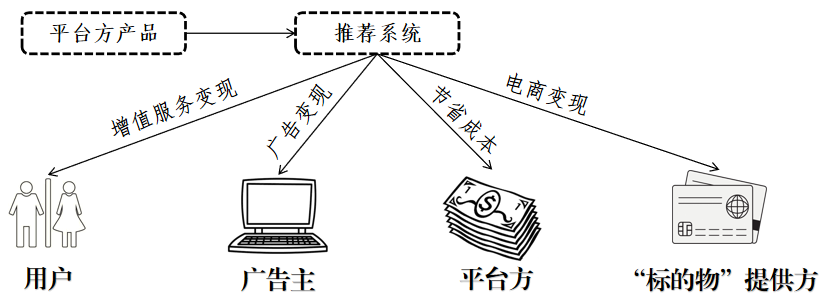
\includegraphics[width=0.95\textwidth]{1}
		\caption{推荐系统与互联网融合体现的经济价值}
		\label{fig:circuit-diagcam}
	\end{figure}
	$\bigstar$\textbf{广告变现:}用户方产品在互联网上投放广告,通过提高广告曝光以及用户点击广告获取权益。通过推荐系统的应用,可以在新闻APP中实现广告精准投放。广告业务偏轻公司一般都会选择流量外包方式做广告变现,\textbf{通过推荐系统提高广告精准投放率与用户点击率即是一种非常好的方式。}\par
	$\bigstar$\textbf{增值服务变现:}增值服务主要是指基本服务以外的特色服务,如新闻平台常见的会员制。推荐系统通过精准把握用户兴趣,引导用户购买会员增值服务产品。推荐系统的个性化推荐服务不仅可以更加深层次的挖掘用户需求,还可以使更多相对冷门但优质的内容得到曝光与展示。在 2004 年,一位杂志主编在形容亚马逊和 Netflix 的商业模式时首次提出“长尾”概念,指代需求和销量不高的产品在市场中所占比例与主流产品相当甚至更高。当传统的二八定律无法再创造更多利润时,商家开始关注“长尾”潜在的商业价值,即专注于小众群体的个性化偏好。\textbf{推荐算法在实现企业从二八定律向“长尾效应”转变方面发挥着重要作用。}以往市场只关注大众需求,而通过推荐系统,个性化需求也可以得到满足,提高了用户的满意程度和消费质量,实现了双赢。\par
	$\bigstar$\textbf{节省成本变现:}在推荐算法还不作为推荐系统的重要组成部分之前,推荐这项工作的大部分还是由人工完成的,根据一些专业人士的建议和想法,来向用户推荐产品及服务。推荐系统对平台方的贡献不仅在于直接的商业价值或是促进用户粘性、用户数量增长等,还可以\textbf{用更少的成本实现最大程度的个性化新闻推荐,提高内容的分发效率。}\par
	$\bigstar$\textbf{电商变现:}无论是传统意义的实体电商产品,还是网络小说、网络课程等虚拟电商产品,都可以通过提高分发商品效率,精准化投放促进商品售卖而提高商家分成,吸引商家入驻。总的来说,\textbf{在电商变现方面,推荐系统可以做到促进“标的物”提供方的生态逐步健全繁荣,获取更多经济效益。}\par
	\subsubsection{ 响应国家发展和改革委员会“新基建”号召}
	国家发改委于2020年4月首次明确了新型基础设施的范围包括以人工智能、云计算、区块链等为代表的新技术基础设施,新型基础设施建设对于打造经济新动能、重塑供应新链条、促进惠民新模式有重大意义,是当前稳经济、促增长的核心支撑。人工智能、云计算、物联网等现代信息科技依托新型基础设施建设得到了高速发展。\par
	特别是处于疫情后时代,线下娱乐受到重创,线上娱乐成为青年群体最重要的娱乐方式之一。在当前的时代背景下,推荐系统的研究有助于\textbf{促进青年群体的幸福感,扩大新型基础设施建设的有效投资,有效对冲经济下行压力,有力支撑经济社会高质量恢复与持续发展。}
	\subsection{相关研究现状}
	推荐系统是学术界和工业界研究的热门话题。学术界侧重理论层面的分析和模型性能的提升,而工业界更侧重实践层面的发展以及用户体验的提升以及推荐系统的应用前景。下面从这两方面分别介绍。
	\subsubsection{ 推荐系统在工业界的应用与发展前景}
	在移动互联网快速发展、智能手机普及以及信息产生爆炸增长的背景下,高效获取对个人有价值的信息变得愈发重要。推荐系统作为一种高效的信息过滤工具,在用户精准高效获取信息方面起到了重要作用。它不仅解决了用户需求不明确时的信息获取问题,也在内容分发、用户体验和商业变现方面发挥着关键作用。推荐系统已经成为toC互联网产品的标配技术,并给应用它的企业带来了丰厚的利润。据报道,推荐系统给亚马逊带来了35\%的销售收入,给Netflix带来了高达75\%的消费,并且Youtube主页上60\%的浏览来自推荐服务。如下表1所示,常见的推荐系统以及推荐内容与使用的特征表,展示了国内应用了推荐系统的常见应用。\par
	\begin{table}[H]
		\centering
		\caption{不同推荐场景下的推荐内容和特征}
		\begin{tabular}{|m{2cm}|m{4cm}|m{4cm}|m{4cm}|}
			\hline
			推荐场景 & 推荐产品 & 推荐项 & 推荐使用的特征 \\
			\hline
			资讯推荐 & 今日头条、百度新闻、腾讯新闻、知乎 & 新闻标题、内容、主题 & 用户行为、用户画像、年龄、性别、教育背景 \\
			\hline
			快资讯 & 抖音、快手、西瓜视频、YouTube & 视频内容、音频、类型 & 热度、标题和描述、用户行为 \\
			\hline
			腾讯视频 & 爱奇艺、优酷、HBO、Netflix & QQ音乐、网易云音乐 & 音频类型、演唱者、作曲者等 \\
			\hline
			电商推荐 & 淘宝、京东、亚马逊、拼多多 & 商品 & 商品标题、描述、图片、类别、流行度 \\
			\hline
		\end{tabular}
	\end{table}
	推荐系统的发展与大环境和技术进步密不可分,接下来我们从三个层面分析推荐系统发展的前景:\par
	$\bigstar$\textbf{政策层面:}在当前“智能化”的时代背景下,国家空前把人工智能提升到了战略的高度,政策的大力支持、媒体的大肆宣扬以及样板示范作用,让个性化新闻推荐的产品与业务受到了更多投资人、专家的重视,这不仅极大推动了新闻推荐系统的发展,也有利于推荐系统在更多的业务场景下落地。\par
	$\bigstar$\textbf{教育层面:}国内从2016年起步开始开设数据科学与大数据技术、智能科学与技术等人工智能相关专业,推荐系统作为大数据和人工智能领域业务价值最大之一的领域,极大的受益于大数据与人工智能相关学科人才的增长,这为助力推荐系统进一步发展提供了基础。\par
	$\bigstar$\textbf{科技层面:}构建一套灵活实时、准确度高、稳定高效的新闻推荐系统是非常困难的,它不仅涉及到业务场景,还与产品交互、工程应用密不可分,几乎只有中、大规模的公司才会构建一套推荐算法业务体系,但受益于云计算基础设施的逐步健全,创业公司可以利用云平台提供的SAAS服务搭建自己的推荐系统模块,降低了推荐系统的使用门槛,促进了推荐系统更加广泛的应用。\par
	\subsubsection{ 推荐系统在学术界的研究现状}
	根据用户日志的数据的输入形式和推荐算法的设计机制,推荐系统在学术界的发展主要包含以下三个阶段:基于协同过滤的推荐、基于内容的推荐以及混合推荐。\par
	$\bullet$\textbf{基于协同过滤的推荐:}协同过滤推荐算法是诞生最早且比较著名的推荐算法,这种算法主要考虑了用户与与用户之间的相似度,在所有用户群体中找到与用户具有相似兴趣、相似偏好的的用户感兴趣的产品或服务推荐给用户。例如下图3中的情景,小林喜欢《间谍过家家》和《干物妹小埋》这类喜剧动漫片,小浩也喜欢看喜剧动漫,如《间谍过家家》、《干物妹小埋》和《工作细胞》等。基于相似喜好,在协同过滤算法中会将小林未看过但小浩喜欢的电影《工作细胞》推荐给小林。\par
	\begin{figure}[H]
		\centering
		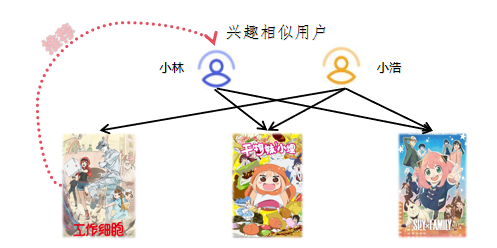
\includegraphics[width=0.65\textwidth]{3}
		\caption{协同过滤推荐示例}
		\label{fig:circuit-diagcam}
	\end{figure}
	目前学术界已提出多种协同过滤的推荐算法,包括传统的矩阵分解方法和结合深度学习技术的新型方法。传统方法存在冷启动和数据稀疏等问题,而深度学习结合的方法如Autoencoders、CDAE和DMF能更好地解决这些问题,通过学习用户和项的潜在因子来提高推荐性能。尽管协同过滤在工业界得到广泛应用,但仍面临冷启动等挑战,需要进一步研究完善。\par
	$\bullet$\textbf{基于内容的推荐:}这种算法不同于协同过滤算法,根据用户的交互记录为用户提供个性化推荐结果,基于内容的推荐算法的基本原理是根据用户和项的属性特征以及用户的历史行为,获得用户的兴趣偏好,为用户推荐跟他的兴趣偏好相匹配的项。例如小琰经常浏览与各地旅游攻略相关的资讯,基于内容的推荐算法则可能推荐近期爆火的旅游地相关新闻。\par
	基于内容的推荐方法早期采用统计策略,如TF-IDF和余弦相似度,存在内容相同但物品不同的问题。后续方法利用机器学习技术如决策树、最近邻居和神经网络解决这一问题,比如DeepWide和DeepFM。目前主流的基于深度神经网络的推荐算法使用CNN、RNN、注意力网络或记忆网络从用户历史交互序列中提取特征,例如DeepJoNN、ATEM和MANN。为克服错误关系假设,一些方法利用神经网络挖掘用户的长期兴趣和短期兴趣,融合长短期兴趣做个性化推荐,这称为以会话为主的推荐方法。\par
	$\bullet$\textbf{混合推荐:}混合推荐算法进一步提升了推荐系统的性能,融合了知识图谱的信息,增加了推荐系统内部算法的可解释性。利用知识表示学习技术将丰富语义信息融入推荐过程,使结果更准确满足用户需求。混合推荐方法建立用户知识图谱,利用路径推理、强化学习和图神经网络技术将购买关系建模为知识图谱的补全任务,从中学习用户和项的表示并预测匹配概率,即向用户推荐该项的概率。比如较为经典的 KPRN 方法使用循环神经网络挖掘用户与物品之间的图谱路径,利用知识图谱的路径推理技术建模用户与候选推荐项的可解释性推荐。这一前沿技术解决了推荐算法黑盒问题,提高了推荐结果的可解释性,是未来推荐系统的重要研究方向。\par
	表 2 列举了上述三类方法的经典模型、各模型使用的核心技术以及评测指标等。
	\begin{table}[H]
	\centering
	\caption{三类方法的核心技术对比}
	\begin{tabular}{|m{2cm}|m{4cm}|m{4cm}|m{4cm}|}
		\hline
		推荐场景 & 方法举例 & 核心技术 & 评价指标 \\
		\hline
		协同过滤推荐方法 & Autoencoders、CADE、DMF、CKE & 矩阵分解、张量分解、神经网络 & accuracy、MRR、ndcg@k \\
		\hline
		基于文本内容推荐 & TransRec、DeepCoNN、JRL、DKN、DAN & 卷积神经网络、循环神经网络、注意力机制 & accuracy、MRR、ndcg@k \\
		\hline
		混合推荐方法 & KPRN、RippleNet、KGCN、VGAE、PGPR & 强化学习、图卷积神经网络、深度神经网络、注意力神经网络 & accuracy、MRR、ndcg@k \\
		\hline
	\end{tabular}
\end{table}
	\subsection{项目架构总览}
	\subsubsection{ 项目整体框架}
	\begin{figure}[H]
		\centering
		\includegraphics[width=0.95\textwidth]{MGCA}
		\caption{MGCA推荐系统算法框架}
		\label{fig:circuit-diagcam}
	\end{figure}
	\subsubsection{ 项目优势与创新性}
	\newpage
	\section{模型技术路线及实现方案}
	\subsection{数据集选取}
	\subsubsection{ MIND数据集}
	\subsubsection{ glove词嵌入}
	\subsubsection{ 数据预处理}
	\subsection{方法介绍}
	\subsubsection{ 图神经网络}
	\subsubsection{ 注意力机制}
	\subsubsection{ Transformer}
	\subsubsection{ Fastformer}
	\subsection{模型架构}
	\subsubsection{ 总体架构}
	\subsubsection{ 候选新闻编码}
	\subsubsection{ 单词粒度感知候选新闻}
	\subsubsection{ 新闻粒度感知候选新闻}
	\subsubsection{ 实体粒度感知候选新闻}
	\subsection{模型评估}
	\subsubsection{ 与之前模型的性能对比}
	\subsubsection{ 消融实验}
	\newpage
	\section{软件工程与开发架构方案}
	\subsection{开发工具与框架}
	\subsection{新闻推荐系统软件落地示例}
	\subsubsection{ 软件周期模型}
	\subsubsection{ 软件开发模型}
	\subsubsection{ 数据库设计}
	\subsubsection{ UML设计}
	\subsubsection{ 软件功能演示}
	\subsubsection{ 兼容性测试与稳定性测试}
	$\bigstar$可执行测试:分别部署到不同性能的电脑上运行测试,均成功运行,网页反馈
	均在35ms到45ms左右,不存在延迟和卡顿现象,该系统对电脑的配置要求较低。\par
	$\bigstar$功能测试:所有功能均可正常运行使用,可视化动态大屏显示正常,首页展示
	效果正常,查询功能正常,链接页面跳转正常。\par
	$\bigstar$兼容测试:在 Windows、Linux、Mac等操作系统可以正常访问。谷歌浏览器、
	火狐浏览器、QQ 浏览器、360 浏览器等运行均正常。Windows操作系统的python版
	本为3.6以上、tensorflow2.14.0 版本环境可以正常运行平台。\par
	$\bigstar$安全测试:本项目采取的是 https 协议,安全性和可靠性比较高,jupyter 环境
	提供了三种安全级服务配置,可以按照实际的需求提升安全等级。\par
	\newpage
	\section{商业模式构建与经营管理}
	\subsection{市场竞争分析}
	\subsection{投资回报分析}
	\subsection{盈利方式}
	\subsubsection{ 提供整套低耦合工业界解决方案}
	\subsubsection{ 提供整套成熟软件系统}
	\subsection{财务管理}
	\subsection{营销战略}
	\newpage
	
	%参考文献
	\begin{thebibliography}{9}%宽度9
		[1]陈昌凤,袁雨晴.智能新闻业:生成式人工智能成为基础设施[J].内蒙古社会科学,2024,45(01):40-48.DOI:10.14137/j.cnki.issn1003-5281.2024.01.006.
	\end{thebibliography}
	
	\newpage
\end{document}
